\documentclass[1p]{elsarticle_modified}
%\bibliographystyle{elsarticle-num}

%\usepackage[colorlinks]{hyperref}
%\usepackage{abbrmath_seonhwa} %\Abb, \Ascr, \Acal ,\Abf, \Afrak
\usepackage{amsfonts}
\usepackage{amssymb}
\usepackage{amsmath}
\usepackage{amsthm}
\usepackage{scalefnt}
\usepackage{amsbsy}
\usepackage{kotex}
\usepackage{caption}
\usepackage{subfig}
\usepackage{color}
\usepackage{graphicx}
\usepackage{xcolor} %% white, black, red, green, blue, cyan, magenta, yellow
\usepackage{float}
\usepackage{setspace}
\usepackage{hyperref}

\usepackage{tikz}
\usetikzlibrary{arrows}

\usepackage{multirow}
\usepackage{array} % fixed length table
\usepackage{hhline}

%%%%%%%%%%%%%%%%%%%%%
\makeatletter
\renewcommand*\env@matrix[1][\arraystretch]{%
	\edef\arraystretch{#1}%
	\hskip -\arraycolsep
	\let\@ifnextchar\new@ifnextchar
	\array{*\c@MaxMatrixCols c}}
\makeatother %https://tex.stackexchange.com/questions/14071/how-can-i-increase-the-line-spacing-in-a-matrix
%%%%%%%%%%%%%%%

\usepackage[normalem]{ulem}

\newcommand{\msout}[1]{\ifmmode\text{\sout{\ensuremath{#1}}}\else\sout{#1}\fi}
%SOURCE: \msout is \stkout macro in https://tex.stackexchange.com/questions/20609/strikeout-in-math-mode

\newcommand{\cancel}[1]{
	\ifmmode
	{\color{red}\msout{#1}}
	\else
	{\color{red}\sout{#1}}
	\fi
}

\newcommand{\add}[1]{
	{\color{blue}\uwave{#1}}
}

\newcommand{\replace}[2]{
	\ifmmode
	{\color{red}\msout{#1}}{\color{blue}\uwave{#2}}
	\else
	{\color{red}\sout{#1}}{\color{blue}\uwave{#2}}
	\fi
}

\newcommand{\Sol}{\mathcal{S}} %segment
\newcommand{\D}{D} %diagram
\newcommand{\A}{\mathcal{A}} %arc


%%%%%%%%%%%%%%%%%%%%%%%%%%%%%5 test

\def\sl{\operatorname{\textup{SL}}(2,\Cbb)}
\def\psl{\operatorname{\textup{PSL}}(2,\Cbb)}
\def\quan{\mkern 1mu \triangleright \mkern 1mu}

\theoremstyle{definition}
\newtheorem{thm}{Theorem}[section]
\newtheorem{prop}[thm]{Proposition}
\newtheorem{lem}[thm]{Lemma}
\newtheorem{ques}[thm]{Question}
\newtheorem{cor}[thm]{Corollary}
\newtheorem{defn}[thm]{Definition}
\newtheorem{exam}[thm]{Example}
\newtheorem{rmk}[thm]{Remark}
\newtheorem{alg}[thm]{Algorithm}

\newcommand{\I}{\sqrt{-1}}
\begin{document}

%\begin{frontmatter}
%
%\title{Boundary parabolic representations of knots up to 8 crossings}
%
%%% Group authors per affiliation:
%\author{Yunhi Cho} 
%\address{Department of Mathematics, University of Seoul, Seoul, Korea}
%\ead{yhcho@uos.ac.kr}
%
%
%\author{Seonhwa Kim} %\fnref{s_kim}}
%\address{Center for Geometry and Physics, Institute for Basic Science, Pohang, 37673, Korea}
%\ead{ryeona17@ibs.re.kr}
%
%\author{Hyuk Kim}
%\address{Department of Mathematical Sciences, Seoul National University, Seoul 08826, Korea}
%\ead{hyukkim@snu.ac.kr}
%
%\author{Seokbeom Yoon}
%\address{Department of Mathematical Sciences, Seoul National University, Seoul, 08826,  Korea}
%\ead{sbyoon15@snu.ac.kr}
%
%\begin{abstract}
%We find all boundary parabolic representation of knots up to 8 crossings.
%
%\end{abstract}
%\begin{keyword}
%    \MSC[2010] 57M25 
%\end{keyword}
%
%\end{frontmatter}

%\linenumbers
%\tableofcontents
%
\newcommand\colored[1]{\textcolor{white}{\rule[-0.35ex]{0.8em}{1.4ex}}\kern-0.8em\color{red} #1}%
%\newcommand\colored[1]{\textcolor{white}{ #1}\kern-2.17ex	\textcolor{white}{ #1}\kern-1.81ex	\textcolor{white}{ #1}\kern-2.15ex\color{red}#1	}

{\Large $\underline{12a_{0730}~(K12a_{0730})}$}

\setlength{\tabcolsep}{10pt}
\renewcommand{\arraystretch}{1.6}
\vspace{1cm}\begin{tabular}{m{100pt}>{\centering\arraybackslash}m{274pt}}
\multirow{5}{120pt}{
	\centering
	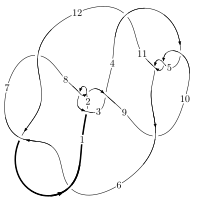
\includegraphics[width=112pt]{../../../GIT/diagram.site/Diagrams/png/1531_12a_0730.png}\\
\ \ \ A knot diagram\footnotemark}&
\allowdisplaybreaks
\textbf{Linearized knot diagam} \\
\cline{2-2}
 &
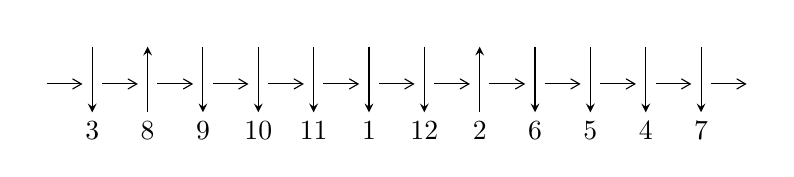
\begin{tikzpicture}[x=20pt, y=17pt]
	% nodes
	\node (C0) at (0, 0) {};
	\node (C1) at (1, 0) {};
	\node (C1U) at (1, +1) {};
	\node (C1D) at (1, -1) {3};

	\node (C2) at (2, 0) {};
	\node (C2U) at (2, +1) {};
	\node (C2D) at (2, -1) {8};

	\node (C3) at (3, 0) {};
	\node (C3U) at (3, +1) {};
	\node (C3D) at (3, -1) {9};

	\node (C4) at (4, 0) {};
	\node (C4U) at (4, +1) {};
	\node (C4D) at (4, -1) {10};

	\node (C5) at (5, 0) {};
	\node (C5U) at (5, +1) {};
	\node (C5D) at (5, -1) {11};

	\node (C6) at (6, 0) {};
	\node (C6U) at (6, +1) {};
	\node (C6D) at (6, -1) {1};

	\node (C7) at (7, 0) {};
	\node (C7U) at (7, +1) {};
	\node (C7D) at (7, -1) {12};

	\node (C8) at (8, 0) {};
	\node (C8U) at (8, +1) {};
	\node (C8D) at (8, -1) {2};

	\node (C9) at (9, 0) {};
	\node (C9U) at (9, +1) {};
	\node (C9D) at (9, -1) {6};

	\node (C10) at (10, 0) {};
	\node (C10U) at (10, +1) {};
	\node (C10D) at (10, -1) {5};

	\node (C11) at (11, 0) {};
	\node (C11U) at (11, +1) {};
	\node (C11D) at (11, -1) {4};

	\node (C12) at (12, 0) {};
	\node (C12U) at (12, +1) {};
	\node (C12D) at (12, -1) {7};
	\node (C13) at (13, 0) {};

	% arrows
	\draw[->,>={angle 60}]
	(C0) edge (C1) (C1) edge (C2) (C2) edge (C3) (C3) edge (C4) (C4) edge (C5) (C5) edge (C6) (C6) edge (C7) (C7) edge (C8) (C8) edge (C9) (C9) edge (C10) (C10) edge (C11) (C11) edge (C12) (C12) edge (C13) ;	\draw[->,>=stealth]
	(C1U) edge (C1D) (C2D) edge (C2U) (C3U) edge (C3D) (C4U) edge (C4D) (C5U) edge (C5D) (C6U) edge (C6D) (C7U) edge (C7D) (C8D) edge (C8U) (C9U) edge (C9D) (C10U) edge (C10D) (C11U) edge (C11D) (C12U) edge (C12D) ;
	\end{tikzpicture} \\
\hhline{~~} \\& 
\textbf{Solving Sequence} \\ \cline{2-2} 
 &
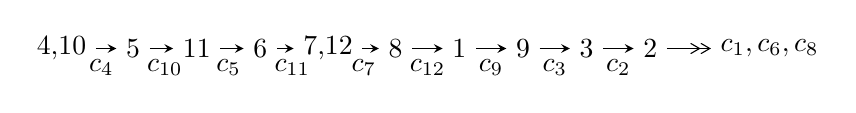
\begin{tikzpicture}[x=23pt, y=7pt]
	% node
	\node (A0) at (-1/8, 0) {4,10};
	\node (A1) at (1, 0) {5};
	\node (A2) at (2, 0) {11};
	\node (A3) at (3, 0) {6};
	\node (A4) at (65/16, 0) {7,12};
	\node (A5) at (41/8, 0) {8};
	\node (A6) at (49/8, 0) {1};
	\node (A7) at (57/8, 0) {9};
	\node (A8) at (65/8, 0) {3};
	\node (A9) at (73/8, 0) {2};
	\node (C1) at (1/2, -1) {$c_{4}$};
	\node (C2) at (3/2, -1) {$c_{10}$};
	\node (C3) at (5/2, -1) {$c_{5}$};
	\node (C4) at (7/2, -1) {$c_{11}$};
	\node (C5) at (37/8, -1) {$c_{7}$};
	\node (C6) at (45/8, -1) {$c_{12}$};
	\node (C7) at (53/8, -1) {$c_{9}$};
	\node (C8) at (61/8, -1) {$c_{3}$};
	\node (C9) at (69/8, -1) {$c_{2}$};
	\node (A10) at (11, 0) {$c_{1},c_{6},c_{8}$};

	% edge
	\draw[->,>=stealth]	
	(A0) edge (A1) (A1) edge (A2) (A2) edge (A3) (A3) edge (A4) (A4) edge (A5) (A5) edge (A6) (A6) edge (A7) (A7) edge (A8) (A8) edge (A9) ;
	\draw[->>,>={angle 60}]	
	(A9) edge (A10);
\end{tikzpicture} \\ 

\end{tabular} \\

\footnotetext{
The image of knot diagram is generated by the software ``\textbf{Draw programme}" developed by Andrew Bartholomew(\url{http://www.layer8.co.uk/maths/draw/index.htm\#Running-draw}), where we modified some parts for our purpose(\url{https://github.com/CATsTAILs/LinksPainter}).
}\phantom \\ \newline 
\centering \textbf{Ideals for irreducible components\footnotemark of $X_{\text{par}}$} 
 
\begin{align*}
I^u_{1}&=\langle 
u^{55}-23 u^{53}+\cdots+4 b+2 u,\;u^{53}-22 u^{51}+\cdots+4 a-4,\;u^{58}+2 u^{57}+\cdots- u+2\rangle \\
I^u_{2}&=\langle 
2093 u^7 a^2-394 u^7 a+\cdots+1311 a-1282,\;2 u^7 a^2-4 u^7 a+\cdots+6 a-1,\\
\phantom{I^u_{2}}&\phantom{= \langle  }u^8- u^7-3 u^6+2 u^5+3 u^4-2 u-1\rangle \\
I^u_{3}&=\langle 
- u^5+u^4+2 u^3-2 u^2+b- u,\;u^5-3 u^3+a+2 u,\;u^6-3 u^4+2 u^2+1\rangle \\
\\
\end{align*}
\raggedright * 3 irreducible components of $\dim_{\mathbb{C}}=0$, with total 88 representations.\\
\footnotetext{All coefficients of polynomials are rational numbers. But the coefficients are sometimes approximated in decimal forms when there is not enough margin.}
\newpage
\renewcommand{\arraystretch}{1}
\centering \section*{I. $I^u_{1}= \langle u^{55}-23 u^{53}+\cdots+4 b+2 u,\;u^{53}-22 u^{51}+\cdots+4 a-4,\;u^{58}+2 u^{57}+\cdots- u+2 \rangle$}
\flushleft \textbf{(i) Arc colorings}\\
\begin{tabular}{m{7pt} m{180pt} m{7pt} m{180pt} }
\flushright $a_{4}=$&$\begin{pmatrix}1\\0\end{pmatrix}$ \\
\flushright $a_{10}=$&$\begin{pmatrix}0\\u\end{pmatrix}$ \\
\flushright $a_{5}=$&$\begin{pmatrix}1\\u^2\end{pmatrix}$ \\
\flushright $a_{11}=$&$\begin{pmatrix}- u\\- u^3+u\end{pmatrix}$ \\
\flushright $a_{6}=$&$\begin{pmatrix}- u^2+1\\- u^4+2 u^2\end{pmatrix}$ \\
\flushright $a_{7}=$&$\begin{pmatrix}-\frac{1}{4} u^{53}+\frac{11}{2} u^{51}+\cdots+\frac{1}{4} u+1\\-\frac{1}{4} u^{55}+\frac{23}{4} u^{53}+\cdots+\frac{5}{2} u^2-\frac{1}{2} u\end{pmatrix}$ \\
\flushright $a_{12}=$&$\begin{pmatrix}u^3-2 u\\- u^3+u\end{pmatrix}$ \\
\flushright $a_{8}=$&$\begin{pmatrix}\frac{1}{2} u^{57}+u^{56}+\cdots+\frac{1}{4} u+1\\- u^{57}- u^{56}+\cdots+\frac{1}{2} u-1\end{pmatrix}$ \\
\flushright $a_{1}=$&$\begin{pmatrix}\frac{1}{4} u^{54}-\frac{23}{4} u^{52}+\cdots-\frac{5}{2} u+\frac{1}{2}\\-\frac{1}{4} u^{54}+\frac{11}{2} u^{52}+\cdots+\frac{1}{4} u^2+u\end{pmatrix}$ \\
\flushright $a_{9}=$&$\begin{pmatrix}u^5-2 u^3+u\\u^7-3 u^5+2 u^3+u\end{pmatrix}$ \\
\flushright $a_{3}=$&$\begin{pmatrix}- u^{12}+5 u^{10}-9 u^8+6 u^6- u^2+1\\- u^{14}+6 u^{12}-13 u^{10}+10 u^8+2 u^6-4 u^4- u^2\end{pmatrix}$ \\
\flushright $a_{2}=$&$\begin{pmatrix}-\frac{1}{4} u^{51}+\frac{11}{2} u^{49}+\cdots-\frac{9}{4} u+1\\\frac{1}{4} u^{51}-\frac{21}{4} u^{49}+\cdots-\frac{1}{2} u^2+\frac{1}{2} u\end{pmatrix}$\\&\end{tabular}
\flushleft \textbf{(ii) Obstruction class $= -1$}\\~\\
\flushleft \textbf{(iii) Cusp Shapes $= -2 u^{57}+48 u^{55}+\cdots+10 u^2-14$}\\~\\
\newpage\renewcommand{\arraystretch}{1}
\flushleft \textbf{(iv) u-Polynomials at the component}\newline \\
\begin{tabular}{m{50pt}|m{274pt}}
Crossings & \hspace{64pt}u-Polynomials at each crossing \\
\hline $$\begin{aligned}c_{1}\end{aligned}$$&$\begin{aligned}
&u^{58}+27 u^{57}+\cdots+240 u+25
\end{aligned}$\\
\hline $$\begin{aligned}c_{2},c_{8}\end{aligned}$$&$\begin{aligned}
&u^{58}- u^{57}+\cdots-10 u+5
\end{aligned}$\\
\hline $$\begin{aligned}c_{3}\end{aligned}$$&$\begin{aligned}
&u^{58}-2 u^{57}+\cdots-18880 u+3200
\end{aligned}$\\
\hline $$\begin{aligned}c_{4},c_{5},c_{10}\end{aligned}$$&$\begin{aligned}
&u^{58}+2 u^{57}+\cdots- u+2
\end{aligned}$\\
\hline $$\begin{aligned}c_{6},c_{7},c_{12}\end{aligned}$$&$\begin{aligned}
&u^{58}- u^{57}+\cdots-32 u+5
\end{aligned}$\\
\hline $$\begin{aligned}c_{9},c_{11}\end{aligned}$$&$\begin{aligned}
&u^{58}-6 u^{57}+\cdots-608 u+128
\end{aligned}$\\
\hline
\end{tabular}\\~\\
\newpage\renewcommand{\arraystretch}{1}
\flushleft \textbf{(v) Riley Polynomials at the component}\newline \\
\begin{tabular}{m{50pt}|m{274pt}}
Crossings & \hspace{64pt}Riley Polynomials at each crossing \\
\hline $$\begin{aligned}c_{1}\end{aligned}$$&$\begin{aligned}
&y^{58}+15 y^{57}+\cdots+14700 y+625
\end{aligned}$\\
\hline $$\begin{aligned}c_{2},c_{8}\end{aligned}$$&$\begin{aligned}
&y^{58}+27 y^{57}+\cdots+240 y+25
\end{aligned}$\\
\hline $$\begin{aligned}c_{3}\end{aligned}$$&$\begin{aligned}
&y^{58}-18 y^{57}+\cdots-108646400 y+10240000
\end{aligned}$\\
\hline $$\begin{aligned}c_{4},c_{5},c_{10}\end{aligned}$$&$\begin{aligned}
&y^{58}-48 y^{57}+\cdots+19 y+4
\end{aligned}$\\
\hline $$\begin{aligned}c_{6},c_{7},c_{12}\end{aligned}$$&$\begin{aligned}
&y^{58}+55 y^{57}+\cdots-624 y+25
\end{aligned}$\\
\hline $$\begin{aligned}c_{9},c_{11}\end{aligned}$$&$\begin{aligned}
&y^{58}+32 y^{57}+\cdots+31744 y+16384
\end{aligned}$\\
\hline
\end{tabular}\\~\\
\newpage\flushleft \textbf{(vi) Complex Volumes and Cusp Shapes}
$$\begin{array}{c|c|c}  
\text{Solutions to }I^u_{1}& \I (\text{vol} + \sqrt{-1}CS) & \text{Cusp shape}\\
 \hline 
\begin{aligned}
u &= -1.055470 + 0.361002 I \\
a &= \phantom{-}1.72697 - 1.44530 I \\
b &= -1.84334 - 1.14825 I\end{aligned}
 & \phantom{-}2.13911 - 7.31160 I & \phantom{-0.000000 } 0 \\ \hline\begin{aligned}
u &= -1.055470 - 0.361002 I \\
a &= \phantom{-}1.72697 + 1.44530 I \\
b &= -1.84334 + 1.14825 I\end{aligned}
 & \phantom{-}2.13911 + 7.31160 I & \phantom{-0.000000 } 0 \\ \hline\begin{aligned}
u &= \phantom{-}1.079220 + 0.287984 I \\
a &= -0.543736 - 0.144608 I \\
b &= \phantom{-}0.874982 - 0.215155 I\end{aligned}
 & -3.05587 + 3.30062 I & \phantom{-0.000000 } 0 \\ \hline\begin{aligned}
u &= \phantom{-}1.079220 - 0.287984 I \\
a &= -0.543736 + 0.144608 I \\
b &= \phantom{-}0.874982 + 0.215155 I\end{aligned}
 & -3.05587 - 3.30062 I & \phantom{-0.000000 } 0 \\ \hline\begin{aligned}
u &= \phantom{-}1.113240 + 0.346536 I \\
a &= \phantom{-}1.83136 + 1.57124 I \\
b &= -2.11612 + 1.33467 I\end{aligned}
 & \phantom{-}4.49527 + 1.92718 I & \phantom{-0.000000 } 0 \\ \hline\begin{aligned}
u &= \phantom{-}1.113240 - 0.346536 I \\
a &= \phantom{-}1.83136 - 1.57124 I \\
b &= -2.11612 - 1.33467 I\end{aligned}
 & \phantom{-}4.49527 - 1.92718 I & \phantom{-0.000000 } 0 \\ \hline\begin{aligned}
u &= -0.160239 + 0.809860 I \\
a &= -3.28036 + 1.61495 I \\
b &= \phantom{-}2.76593 - 0.91652 I\end{aligned}
 & \phantom{-}4.87856 + 11.59130 I & -4.05373 - 7.92500 I \\ \hline\begin{aligned}
u &= -0.160239 - 0.809860 I \\
a &= -3.28036 - 1.61495 I \\
b &= \phantom{-}2.76593 + 0.91652 I\end{aligned}
 & \phantom{-}4.87856 - 11.59130 I & -4.05373 + 7.92500 I \\ \hline\begin{aligned}
u &= \phantom{-}0.022956 + 0.824654 I \\
a &= -4.22626 - 0.30258 I \\
b &= \phantom{-}3.31540 + 0.17209 I\end{aligned}
 & \phantom{-}10.56110 - 2.82315 I & \phantom{-}0.41076 + 3.01430 I \\ \hline\begin{aligned}
u &= \phantom{-}0.022956 - 0.824654 I \\
a &= -4.22626 + 0.30258 I \\
b &= \phantom{-}3.31540 - 0.17209 I\end{aligned}
 & \phantom{-}10.56110 + 2.82315 I & \phantom{-}0.41076 - 3.01430 I\\
 \hline 
 \end{array}$$\newpage$$\begin{array}{c|c|c}  
\text{Solutions to }I^u_{1}& \I (\text{vol} + \sqrt{-1}CS) & \text{Cusp shape}\\
 \hline 
\begin{aligned}
u &= \phantom{-}0.128868 + 0.804285 I \\
a &= -3.63497 - 1.53514 I \\
b &= \phantom{-}2.97126 + 0.87331 I\end{aligned}
 & \phantom{-}7.48930 - 6.12555 I & -0.79979 + 4.12406 I \\ \hline\begin{aligned}
u &= \phantom{-}0.128868 - 0.804285 I \\
a &= -3.63497 + 1.53514 I \\
b &= \phantom{-}2.97126 - 0.87331 I\end{aligned}
 & \phantom{-}7.48930 + 6.12555 I & -0.79979 - 4.12406 I \\ \hline\begin{aligned}
u &= \phantom{-}0.147502 + 0.778831 I \\
a &= \phantom{-}1.128860 + 0.689994 I \\
b &= -0.932523 - 0.020123 I\end{aligned}
 & -0.24972 - 7.28256 I & -7.79026 + 7.04615 I \\ \hline\begin{aligned}
u &= \phantom{-}0.147502 - 0.778831 I \\
a &= \phantom{-}1.128860 - 0.689994 I \\
b &= -0.932523 + 0.020123 I\end{aligned}
 & -0.24972 + 7.28256 I & -7.79026 - 7.04615 I \\ \hline\begin{aligned}
u &= -0.672408 + 0.378683 I \\
a &= \phantom{-}0.49133 + 1.34433 I \\
b &= -0.425204 + 0.224307 I\end{aligned}
 & \phantom{-}1.18428 + 7.12571 I & -7.47098 - 7.52133 I \\ \hline\begin{aligned}
u &= -0.672408 - 0.378683 I \\
a &= \phantom{-}0.49133 - 1.34433 I \\
b &= -0.425204 - 0.224307 I\end{aligned}
 & \phantom{-}1.18428 - 7.12571 I & -7.47098 + 7.52133 I \\ \hline\begin{aligned}
u &= \phantom{-}0.013221 + 0.738470 I \\
a &= \phantom{-}0.751533 - 0.518009 I \\
b &= -0.817557 + 0.051451 I\end{aligned}
 & \phantom{-}3.40366 + 1.43308 I & -1.61750 - 4.02310 I \\ \hline\begin{aligned}
u &= \phantom{-}0.013221 - 0.738470 I \\
a &= \phantom{-}0.751533 + 0.518009 I \\
b &= -0.817557 - 0.051451 I\end{aligned}
 & \phantom{-}3.40366 - 1.43308 I & -1.61750 + 4.02310 I \\ \hline\begin{aligned}
u &= -0.280682 + 0.663131 I \\
a &= \phantom{-}0.264754 + 0.958031 I \\
b &= -0.667970 - 0.059101 I\end{aligned}
 & \phantom{-}2.50446 - 3.37914 I & -4.75082 + 2.18121 I \\ \hline\begin{aligned}
u &= -0.280682 - 0.663131 I \\
a &= \phantom{-}0.264754 - 0.958031 I \\
b &= -0.667970 + 0.059101 I\end{aligned}
 & \phantom{-}2.50446 + 3.37914 I & -4.75082 - 2.18121 I\\
 \hline 
 \end{array}$$\newpage$$\begin{array}{c|c|c}  
\text{Solutions to }I^u_{1}& \I (\text{vol} + \sqrt{-1}CS) & \text{Cusp shape}\\
 \hline 
\begin{aligned}
u &= \phantom{-}1.236100 + 0.370704 I \\
a &= \phantom{-}1.56436 + 2.14598 I \\
b &= -3.06777 + 0.90490 I\end{aligned}
 & \phantom{-}6.81501 - 1.47559 I & \phantom{-0.000000 } 0 \\ \hline\begin{aligned}
u &= \phantom{-}1.236100 - 0.370704 I \\
a &= \phantom{-}1.56436 - 2.14598 I \\
b &= -3.06777 - 0.90490 I\end{aligned}
 & \phantom{-}6.81501 + 1.47559 I & \phantom{-0.000000 } 0 \\ \hline\begin{aligned}
u &= \phantom{-}1.254450 + 0.308524 I \\
a &= \phantom{-}0.014085 - 0.736150 I \\
b &= \phantom{-}0.658157 - 0.385748 I\end{aligned}
 & -0.43433 - 5.22268 I & \phantom{-0.000000 } 0 \\ \hline\begin{aligned}
u &= \phantom{-}1.254450 - 0.308524 I \\
a &= \phantom{-}0.014085 + 0.736150 I \\
b &= \phantom{-}0.658157 + 0.385748 I\end{aligned}
 & -0.43433 + 5.22268 I & \phantom{-0.000000 } 0 \\ \hline\begin{aligned}
u &= \phantom{-}1.287890 + 0.180041 I \\
a &= -0.733143 - 0.305909 I \\
b &= \phantom{-}0.596300 - 0.730533 I\end{aligned}
 & -4.90932 - 2.79468 I & \phantom{-0.000000 } 0 \\ \hline\begin{aligned}
u &= \phantom{-}1.287890 - 0.180041 I \\
a &= -0.733143 + 0.305909 I \\
b &= \phantom{-}0.596300 + 0.730533 I\end{aligned}
 & -4.90932 + 2.79468 I & \phantom{-0.000000 } 0 \\ \hline\begin{aligned}
u &= \phantom{-}0.175184 + 0.669008 I \\
a &= \phantom{-}1.32336 + 0.54960 I \\
b &= -0.906192 + 0.070742 I\end{aligned}
 & -1.76183 + 0.33500 I & -10.67327 + 0.51437 I \\ \hline\begin{aligned}
u &= \phantom{-}0.175184 - 0.669008 I \\
a &= \phantom{-}1.32336 - 0.54960 I \\
b &= -0.906192 - 0.070742 I\end{aligned}
 & -1.76183 - 0.33500 I & -10.67327 - 0.51437 I \\ \hline\begin{aligned}
u &= \phantom{-}0.650108 + 0.232781 I \\
a &= -0.150677 - 0.390107 I \\
b &= \phantom{-}0.732516 + 0.177916 I\end{aligned}
 & -3.55630 - 3.54967 I & -13.4561 + 5.7470 I \\ \hline\begin{aligned}
u &= \phantom{-}0.650108 - 0.232781 I \\
a &= -0.150677 + 0.390107 I \\
b &= \phantom{-}0.732516 - 0.177916 I\end{aligned}
 & -3.55630 + 3.54967 I & -13.4561 - 5.7470 I\\
 \hline 
 \end{array}$$\newpage$$\begin{array}{c|c|c}  
\text{Solutions to }I^u_{1}& \I (\text{vol} + \sqrt{-1}CS) & \text{Cusp shape}\\
 \hline 
\begin{aligned}
u &= -1.283030 + 0.296425 I \\
a &= -0.368173 + 0.033928 I \\
b &= \phantom{-}0.946623 + 0.546835 I\end{aligned}
 & -0.62219 + 2.29529 I & \phantom{-0.000000 } 0 \\ \hline\begin{aligned}
u &= -1.283030 - 0.296425 I \\
a &= -0.368173 - 0.033928 I \\
b &= \phantom{-}0.946623 - 0.546835 I\end{aligned}
 & -0.62219 - 2.29529 I & \phantom{-0.000000 } 0 \\ \hline\begin{aligned}
u &= -1.275740 + 0.370203 I \\
a &= \phantom{-}1.29830 - 2.30847 I \\
b &= -3.30928 - 0.54212 I\end{aligned}
 & \phantom{-}6.52568 + 7.11793 I & \phantom{-0.000000 } 0 \\ \hline\begin{aligned}
u &= -1.275740 - 0.370203 I \\
a &= \phantom{-}1.29830 + 2.30847 I \\
b &= -3.30928 + 0.54212 I\end{aligned}
 & \phantom{-}6.52568 - 7.11793 I & \phantom{-0.000000 } 0 \\ \hline\begin{aligned}
u &= \phantom{-}0.535752 + 0.365918 I \\
a &= \phantom{-}0.36495 - 1.47581 I \\
b &= -0.553992 - 0.181156 I\end{aligned}
 & \phantom{-}3.29520 - 2.38278 I & -4.28188 + 3.63346 I \\ \hline\begin{aligned}
u &= \phantom{-}0.535752 - 0.365918 I \\
a &= \phantom{-}0.36495 + 1.47581 I \\
b &= -0.553992 + 0.181156 I\end{aligned}
 & \phantom{-}3.29520 + 2.38278 I & -4.28188 - 3.63346 I \\ \hline\begin{aligned}
u &= \phantom{-}0.322023 + 0.539515 I \\
a &= \phantom{-}0.085417 - 1.114740 I \\
b &= -0.650618 - 0.010802 I\end{aligned}
 & \phantom{-}4.03344 - 0.91043 I & -2.12378 + 4.36430 I \\ \hline\begin{aligned}
u &= \phantom{-}0.322023 - 0.539515 I \\
a &= \phantom{-}0.085417 + 1.114740 I \\
b &= -0.650618 + 0.010802 I\end{aligned}
 & \phantom{-}4.03344 + 0.91043 I & -2.12378 - 4.36430 I \\ \hline\begin{aligned}
u &= -1.381860 + 0.067257 I \\
a &= \phantom{-}0.298361 - 0.582536 I \\
b &= \phantom{-}1.14365 + 1.03316 I\end{aligned}
 & -2.65450 + 3.62930 I & \phantom{-0.000000 } 0 \\ \hline\begin{aligned}
u &= -1.381860 - 0.067257 I \\
a &= \phantom{-}0.298361 + 0.582536 I \\
b &= \phantom{-}1.14365 - 1.03316 I\end{aligned}
 & -2.65450 - 3.62930 I & \phantom{-0.000000 } 0\\
 \hline 
 \end{array}$$\newpage$$\begin{array}{c|c|c}  
\text{Solutions to }I^u_{1}& \I (\text{vol} + \sqrt{-1}CS) & \text{Cusp shape}\\
 \hline 
\begin{aligned}
u &= -1.354170 + 0.284240 I \\
a &= -0.282971 + 0.964369 I \\
b &= \phantom{-}1.050160 + 0.253647 I\end{aligned}
 & -6.57455 + 3.16360 I & \phantom{-0.000000 } 0 \\ \hline\begin{aligned}
u &= -1.354170 - 0.284240 I \\
a &= -0.282971 - 0.964369 I \\
b &= \phantom{-}1.050160 - 0.253647 I\end{aligned}
 & -6.57455 - 3.16360 I & \phantom{-0.000000 } 0 \\ \hline\begin{aligned}
u &= -1.370230 + 0.194123 I \\
a &= -0.013281 - 0.259852 I \\
b &= \phantom{-}1.010250 + 0.806222 I\end{aligned}
 & -1.25158 + 3.51548 I & \phantom{-0.000000 } 0 \\ \hline\begin{aligned}
u &= -1.370230 - 0.194123 I \\
a &= -0.013281 + 0.259852 I \\
b &= \phantom{-}1.010250 - 0.806222 I\end{aligned}
 & -1.25158 - 3.51548 I & \phantom{-0.000000 } 0 \\ \hline\begin{aligned}
u &= -1.347860 + 0.346662 I \\
a &= \phantom{-}0.54429 - 2.41322 I \\
b &= -3.45164 + 0.39084 I\end{aligned}
 & \phantom{-}2.84200 + 10.27730 I & \phantom{-0.000000 } 0 \\ \hline\begin{aligned}
u &= -1.347860 - 0.346662 I \\
a &= \phantom{-}0.54429 + 2.41322 I \\
b &= -3.45164 - 0.39084 I\end{aligned}
 & \phantom{-}2.84200 - 10.27730 I & \phantom{-0.000000 } 0 \\ \hline\begin{aligned}
u &= -1.355220 + 0.332018 I \\
a &= -0.151021 + 0.986947 I \\
b &= \phantom{-}0.899192 + 0.120955 I\end{aligned}
 & -4.98693 + 11.30040 I & \phantom{-0.000000 } 0 \\ \hline\begin{aligned}
u &= -1.355220 - 0.332018 I \\
a &= -0.151021 - 0.986947 I \\
b &= \phantom{-}0.899192 - 0.120955 I\end{aligned}
 & -4.98693 - 11.30040 I & \phantom{-0.000000 } 0 \\ \hline\begin{aligned}
u &= -1.402640 + 0.030948 I \\
a &= -0.621414 - 0.054979 I \\
b &= -0.624989 + 0.196548 I\end{aligned}
 & -9.84382 + 4.17376 I & \phantom{-0.000000 } 0 \\ \hline\begin{aligned}
u &= -1.402640 - 0.030948 I \\
a &= -0.621414 + 0.054979 I \\
b &= -0.624989 - 0.196548 I\end{aligned}
 & -9.84382 - 4.17376 I & \phantom{-0.000000 } 0\\
 \hline 
 \end{array}$$\newpage$$\begin{array}{c|c|c}  
\text{Solutions to }I^u_{1}& \I (\text{vol} + \sqrt{-1}CS) & \text{Cusp shape}\\
 \hline 
\begin{aligned}
u &= \phantom{-}1.365450 + 0.346164 I \\
a &= \phantom{-}0.39863 + 2.28058 I \\
b &= -3.29230 - 0.55110 I\end{aligned}
 & \phantom{-}0.0648 - 15.7631 I & \phantom{-0.000000 } 0 \\ \hline\begin{aligned}
u &= \phantom{-}1.365450 - 0.346164 I \\
a &= \phantom{-}0.39863 - 2.28058 I \\
b &= -3.29230 + 0.55110 I\end{aligned}
 & \phantom{-}0.0648 + 15.7631 I & \phantom{-0.000000 } 0 \\ \hline\begin{aligned}
u &= \phantom{-}1.387300 + 0.259107 I \\
a &= -0.215334 + 0.244520 I \\
b &= \phantom{-}1.053360 - 0.706502 I\end{aligned}
 & -2.76639 + 0.04256 I & \phantom{-0.000000 } 0 \\ \hline\begin{aligned}
u &= \phantom{-}1.387300 - 0.259107 I \\
a &= -0.215334 - 0.244520 I \\
b &= \phantom{-}1.053360 + 0.706502 I\end{aligned}
 & -2.76639 - 0.04256 I & \phantom{-0.000000 } 0 \\ \hline\begin{aligned}
u &= \phantom{-}1.42580 + 0.05543 I \\
a &= \phantom{-}0.187121 + 0.701410 I \\
b &= \phantom{-}1.22349 - 0.96601 I\end{aligned}
 & -5.43020 - 8.23971 I & \phantom{-0.000000 } 0 \\ \hline\begin{aligned}
u &= \phantom{-}1.42580 - 0.05543 I \\
a &= \phantom{-}0.187121 - 0.701410 I \\
b &= \phantom{-}1.22349 + 0.96601 I\end{aligned}
 & -5.43020 + 8.23971 I & \phantom{-0.000000 } 0 \\ \hline\begin{aligned}
u &= -0.205515 + 0.291758 I \\
a &= \phantom{-}1.197660 + 0.567196 I \\
b &= -0.081785 - 0.431720 I\end{aligned}
 & -0.619748 + 0.918576 I & -10.20880 - 7.11535 I \\ \hline\begin{aligned}
u &= -0.205515 - 0.291758 I \\
a &= \phantom{-}1.197660 - 0.567196 I \\
b &= -0.081785 + 0.431720 I\end{aligned}
 & -0.619748 - 0.918576 I & -10.20880 + 7.11535 I\\
 \hline 
 \end{array}$$\newpage\newpage\renewcommand{\arraystretch}{1}
\centering \section*{II. $I^u_{2}= \langle 2093 u^7 a^2-394 u^7 a+\cdots+1311 a-1282,\;2 u^7 a^2-4 u^7 a+\cdots+6 a-1,\;u^8- u^7-3 u^6+2 u^5+3 u^4-2 u-1 \rangle$}
\flushleft \textbf{(i) Arc colorings}\\
\begin{tabular}{m{7pt} m{180pt} m{7pt} m{180pt} }
\flushright $a_{4}=$&$\begin{pmatrix}1\\0\end{pmatrix}$ \\
\flushright $a_{10}=$&$\begin{pmatrix}0\\u\end{pmatrix}$ \\
\flushright $a_{5}=$&$\begin{pmatrix}1\\u^2\end{pmatrix}$ \\
\flushright $a_{11}=$&$\begin{pmatrix}- u\\- u^3+u\end{pmatrix}$ \\
\flushright $a_{6}=$&$\begin{pmatrix}- u^2+1\\- u^4+2 u^2\end{pmatrix}$ \\
\flushright $a_{7}=$&$\begin{pmatrix}a\\-0.699298 a^{2} u^{7}+0.131640 a u^{7}+\cdots-0.438022 a+0.428333\end{pmatrix}$ \\
\flushright $a_{12}=$&$\begin{pmatrix}u^3-2 u\\- u^3+u\end{pmatrix}$ \\
\flushright $a_{8}=$&$\begin{pmatrix}-0.188774 a^{2} u^{7}+0.106248 a u^{7}+\cdots+0.991647 a-1.14668\\-0.358503 a^{2} u^{7}+0.214166 a u^{7}+\cdots-0.334447 a+1.04711\end{pmatrix}$ \\
\flushright $a_{1}=$&$\begin{pmatrix}0.193451 a^{2} u^{7}+0.438022 a u^{7}+\cdots-0.911794 a+0.668894\\a u\end{pmatrix}$ \\
\flushright $a_{9}=$&$\begin{pmatrix}u^5-2 u^3+u\\u^7-3 u^5+2 u^3+u\end{pmatrix}$ \\
\flushright $a_{3}=$&$\begin{pmatrix}u^3-2 u\\- u^3+u\end{pmatrix}$ \\
\flushright $a_{2}=$&$\begin{pmatrix}0.374206 a^{2} u^{7}-0.458403 a u^{7}+\cdots-0.611761 a-0.222519\\0.558637 a^{2} u^{7}+0.715670 a u^{7}+\cdots-0.320414 a+0.653525\end{pmatrix}$\\&\end{tabular}
\flushleft \textbf{(ii) Obstruction class $= -1$}\\~\\
\flushleft \textbf{(iii) Cusp Shapes $= -4 u^6+12 u^4+4 u^3-8 u^2-8 u-14$}\\~\\
\newpage\renewcommand{\arraystretch}{1}
\flushleft \textbf{(iv) u-Polynomials at the component}\newline \\
\begin{tabular}{m{50pt}|m{274pt}}
Crossings & \hspace{64pt}u-Polynomials at each crossing \\
\hline $$\begin{aligned}c_{1}\end{aligned}$$&$\begin{aligned}
&u^{24}+16 u^{23}+\cdots-4 u+1
\end{aligned}$\\
\hline $$\begin{aligned}c_{2},c_{6},c_{7}\\c_{8},c_{12}\end{aligned}$$&$\begin{aligned}
&u^{24}+8 u^{22}+\cdots-2 u-1
\end{aligned}$\\
\hline $$\begin{aligned}c_{3}\end{aligned}$$&$\begin{aligned}
&(u^8+u^7- u^6-2 u^5+u^4+2 u^3-2 u-1)^3
\end{aligned}$\\
\hline $$\begin{aligned}c_{4},c_{5},c_{10}\end{aligned}$$&$\begin{aligned}
&(u^8- u^7-3 u^6+2 u^5+3 u^4-2 u-1)^3
\end{aligned}$\\
\hline $$\begin{aligned}c_{9},c_{11}\end{aligned}$$&$\begin{aligned}
&(u^8+3 u^7+7 u^6+10 u^5+11 u^4+10 u^3+6 u^2+4 u+1)^3
\end{aligned}$\\
\hline
\end{tabular}\\~\\
\newpage\renewcommand{\arraystretch}{1}
\flushleft \textbf{(v) Riley Polynomials at the component}\newline \\
\begin{tabular}{m{50pt}|m{274pt}}
Crossings & \hspace{64pt}Riley Polynomials at each crossing \\
\hline $$\begin{aligned}c_{1}\end{aligned}$$&$\begin{aligned}
&y^{24}-16 y^{23}+\cdots-20 y+1
\end{aligned}$\\
\hline $$\begin{aligned}c_{2},c_{6},c_{7}\\c_{8},c_{12}\end{aligned}$$&$\begin{aligned}
&y^{24}+16 y^{23}+\cdots-4 y+1
\end{aligned}$\\
\hline $$\begin{aligned}c_{3}\end{aligned}$$&$\begin{aligned}
&(y^8-3 y^7+7 y^6-10 y^5+11 y^4-10 y^3+6 y^2-4 y+1)^3
\end{aligned}$\\
\hline $$\begin{aligned}c_{4},c_{5},c_{10}\end{aligned}$$&$\begin{aligned}
&(y^8-7 y^7+19 y^6-22 y^5+3 y^4+14 y^3-6 y^2-4 y+1)^3
\end{aligned}$\\
\hline $$\begin{aligned}c_{9},c_{11}\end{aligned}$$&$\begin{aligned}
&(y^8+5 y^7+11 y^6+6 y^5-17 y^4-34 y^3-22 y^2-4 y+1)^3
\end{aligned}$\\
\hline
\end{tabular}\\~\\
\newpage\flushleft \textbf{(vi) Complex Volumes and Cusp Shapes}
$$\begin{array}{c|c|c}  
\text{Solutions to }I^u_{2}& \I (\text{vol} + \sqrt{-1}CS) & \text{Cusp shape}\\
 \hline 
\begin{aligned}
u &= -1.180120 + 0.268597 I \\
a &= \phantom{-}0.283758 + 0.634812 I \\
b &= \phantom{-}0.459071 + 0.556325 I\end{aligned}
 & -1.04066 + 1.13123 I & -7.41522 - 0.51079 I \\ \hline\begin{aligned}
u &= -1.180120 + 0.268597 I \\
a &= -0.519143 + 0.133347 I \\
b &= \phantom{-}0.839838 + 0.369976 I\end{aligned}
 & -1.04066 + 1.13123 I & -7.41522 - 0.51079 I \\ \hline\begin{aligned}
u &= -1.180120 + 0.268597 I \\
a &= \phantom{-}2.48773 - 1.66933 I \\
b &= -2.44064 - 2.38764 I\end{aligned}
 & -1.04066 + 1.13123 I & -7.41522 - 0.51079 I \\ \hline\begin{aligned}
u &= -1.180120 - 0.268597 I \\
a &= \phantom{-}0.283758 - 0.634812 I \\
b &= \phantom{-}0.459071 - 0.556325 I\end{aligned}
 & -1.04066 - 1.13123 I & -7.41522 + 0.51079 I \\ \hline\begin{aligned}
u &= -1.180120 - 0.268597 I \\
a &= -0.519143 - 0.133347 I \\
b &= \phantom{-}0.839838 - 0.369976 I\end{aligned}
 & -1.04066 - 1.13123 I & -7.41522 + 0.51079 I \\ \hline\begin{aligned}
u &= -1.180120 - 0.268597 I \\
a &= \phantom{-}2.48773 + 1.66933 I \\
b &= -2.44064 + 2.38764 I\end{aligned}
 & -1.04066 - 1.13123 I & -7.41522 + 0.51079 I \\ \hline\begin{aligned}
u &= -0.108090 + 0.747508 I \\
a &= \phantom{-}0.536114 + 0.684251 I \\
b &= -0.769284 - 0.082442 I\end{aligned}
 & \phantom{-}2.15941 + 2.57849 I & -4.27708 - 3.56796 I \\ \hline\begin{aligned}
u &= -0.108090 + 0.747508 I \\
a &= \phantom{-}1.086910 - 0.593279 I \\
b &= -0.893968 + 0.013597 I\end{aligned}
 & \phantom{-}2.15941 + 2.57849 I & -4.27708 - 3.56796 I \\ \hline\begin{aligned}
u &= -0.108090 + 0.747508 I \\
a &= -4.33823 + 2.20659 I \\
b &= \phantom{-}3.37373 - 1.26294 I\end{aligned}
 & \phantom{-}2.15941 + 2.57849 I & -4.27708 - 3.56796 I \\ \hline\begin{aligned}
u &= -0.108090 - 0.747508 I \\
a &= \phantom{-}0.536114 - 0.684251 I \\
b &= -0.769284 + 0.082442 I\end{aligned}
 & \phantom{-}2.15941 - 2.57849 I & -4.27708 + 3.56796 I\\
 \hline 
 \end{array}$$\newpage$$\begin{array}{c|c|c}  
\text{Solutions to }I^u_{2}& \I (\text{vol} + \sqrt{-1}CS) & \text{Cusp shape}\\
 \hline 
\begin{aligned}
u &= -0.108090 - 0.747508 I \\
a &= \phantom{-}1.086910 + 0.593279 I \\
b &= -0.893968 - 0.013597 I\end{aligned}
 & \phantom{-}2.15941 - 2.57849 I & -4.27708 + 3.56796 I \\ \hline\begin{aligned}
u &= -0.108090 - 0.747508 I \\
a &= -4.33823 - 2.20659 I \\
b &= \phantom{-}3.37373 + 1.26294 I\end{aligned}
 & \phantom{-}2.15941 - 2.57849 I & -4.27708 + 3.56796 I \\ \hline\begin{aligned}
u &= \phantom{-}1.37100\phantom{ +0.000000I} \\
a &= \phantom{-}0.478541 + 0.816744 I \\
b &= \phantom{-}1.31000 - 1.17794 I\end{aligned}
 & -6.50273\phantom{ +0.000000I} & -13.8640\phantom{ +0.000000I} \\ \hline\begin{aligned}
u &= \phantom{-}1.37100\phantom{ +0.000000I} \\
a &= \phantom{-}0.478541 - 0.816744 I \\
b &= \phantom{-}1.31000 + 1.17794 I\end{aligned}
 & -6.50273\phantom{ +0.000000I} & -13.8640\phantom{ +0.000000I} \\ \hline\begin{aligned}
u &= \phantom{-}1.37100\phantom{ +0.000000I} \\
a &= -0.656575\phantom{ +0.000000I} \\
b &= -0.423632\phantom{ +0.000000I}\end{aligned}
 & -6.50273\phantom{ +0.000000I} & -13.8640\phantom{ +0.000000I} \\ \hline\begin{aligned}
u &= \phantom{-}1.334530 + 0.318930 I \\
a &= -0.162462 - 0.927232 I \\
b &= \phantom{-}0.882181 - 0.209095 I\end{aligned}
 & -2.37968 - 6.44354 I & -9.42845 + 5.29417 I \\ \hline\begin{aligned}
u &= \phantom{-}1.334530 + 0.318930 I \\
a &= -0.367019 + 0.108941 I \\
b &= \phantom{-}1.033880 - 0.589591 I\end{aligned}
 & -2.37968 - 6.44354 I & -9.42845 + 5.29417 I \\ \hline\begin{aligned}
u &= \phantom{-}1.334530 + 0.318930 I \\
a &= \phantom{-}0.47028 + 2.85958 I \\
b &= -3.97967 - 0.51225 I\end{aligned}
 & -2.37968 - 6.44354 I & -9.42845 + 5.29417 I \\ \hline\begin{aligned}
u &= \phantom{-}1.334530 - 0.318930 I \\
a &= -0.162462 + 0.927232 I \\
b &= \phantom{-}0.882181 + 0.209095 I\end{aligned}
 & -2.37968 + 6.44354 I & -9.42845 - 5.29417 I \\ \hline\begin{aligned}
u &= \phantom{-}1.334530 - 0.318930 I \\
a &= -0.367019 - 0.108941 I \\
b &= \phantom{-}1.033880 + 0.589591 I\end{aligned}
 & -2.37968 + 6.44354 I & -9.42845 - 5.29417 I\\
 \hline 
 \end{array}$$\newpage$$\begin{array}{c|c|c}  
\text{Solutions to }I^u_{2}& \I (\text{vol} + \sqrt{-1}CS) & \text{Cusp shape}\\
 \hline 
\begin{aligned}
u &= \phantom{-}1.334530 - 0.318930 I \\
a &= \phantom{-}0.47028 - 2.85958 I \\
b &= -3.97967 + 0.51225 I\end{aligned}
 & -2.37968 + 6.44354 I & -9.42845 - 5.29417 I \\ \hline\begin{aligned}
u &= -0.463640\phantom{ +0.000000I} \\
a &= \phantom{-}0.308333\phantom{ +0.000000I} \\
b &= \phantom{-}0.453402\phantom{ +0.000000I}\end{aligned}
 & -0.845036\phantom{ +0.000000I} & -11.8940\phantom{ +0.000000I} \\ \hline\begin{aligned}
u &= -0.463640\phantom{ +0.000000I} \\
a &= \phantom{-}1.21764 + 2.13829 I \\
b &= -0.830005 + 0.371154 I\end{aligned}
 & -0.845036\phantom{ +0.000000I} & -11.8940\phantom{ +0.000000I} \\ \hline\begin{aligned}
u &= -0.463640\phantom{ +0.000000I} \\
a &= \phantom{-}1.21764 - 2.13829 I \\
b &= -0.830005 - 0.371154 I\end{aligned}
 & -0.845036\phantom{ +0.000000I} & -11.8940\phantom{ +0.000000I}\\
 \hline 
 \end{array}$$\newpage\newpage\renewcommand{\arraystretch}{1}
\centering \section*{III. $I^u_{3}= \langle - u^5+u^4+2 u^3-2 u^2+b- u,\;u^5-3 u^3+a+2 u,\;u^6-3 u^4+2 u^2+1 \rangle$}
\flushleft \textbf{(i) Arc colorings}\\
\begin{tabular}{m{7pt} m{180pt} m{7pt} m{180pt} }
\flushright $a_{4}=$&$\begin{pmatrix}1\\0\end{pmatrix}$ \\
\flushright $a_{10}=$&$\begin{pmatrix}0\\u\end{pmatrix}$ \\
\flushright $a_{5}=$&$\begin{pmatrix}1\\u^2\end{pmatrix}$ \\
\flushright $a_{11}=$&$\begin{pmatrix}- u\\- u^3+u\end{pmatrix}$ \\
\flushright $a_{6}=$&$\begin{pmatrix}- u^2+1\\- u^4+2 u^2\end{pmatrix}$ \\
\flushright $a_{7}=$&$\begin{pmatrix}- u^5+3 u^3-2 u\\u^5- u^4-2 u^3+2 u^2+u\end{pmatrix}$ \\
\flushright $a_{12}=$&$\begin{pmatrix}u^3-2 u\\- u^3+u\end{pmatrix}$ \\
\flushright $a_{8}=$&$\begin{pmatrix}- u^5+3 u^3+u^2-2 u-1\\u^5-2 u^3+u\end{pmatrix}$ \\
\flushright $a_{1}=$&$\begin{pmatrix}u^4+u^3-2 u^2-2 u+1\\-1\end{pmatrix}$ \\
\flushright $a_{9}=$&$\begin{pmatrix}u^5-2 u^3+u\\0\end{pmatrix}$ \\
\flushright $a_{3}=$&$\begin{pmatrix}1\\0\end{pmatrix}$ \\
\flushright $a_{2}=$&$\begin{pmatrix}u^4+u^3-2 u^2-2 u+2\\-1\end{pmatrix}$\\&\end{tabular}
\flushleft \textbf{(ii) Obstruction class $= 1$}\\~\\
\flushleft \textbf{(iii) Cusp Shapes $= 4 u^4-8 u^2-8$}\\~\\
\newpage\renewcommand{\arraystretch}{1}
\flushleft \textbf{(iv) u-Polynomials at the component}\newline \\
\begin{tabular}{m{50pt}|m{274pt}}
Crossings & \hspace{64pt}u-Polynomials at each crossing \\
\hline $$\begin{aligned}c_{1}\end{aligned}$$&$\begin{aligned}
&(u-1)^6
\end{aligned}$\\
\hline $$\begin{aligned}c_{2},c_{6},c_{7}\\c_{8},c_{12}\end{aligned}$$&$\begin{aligned}
&(u^2+1)^3
\end{aligned}$\\
\hline $$\begin{aligned}c_{3}\end{aligned}$$&$\begin{aligned}
&u^6
\end{aligned}$\\
\hline $$\begin{aligned}c_{4},c_{5},c_{10}\end{aligned}$$&$\begin{aligned}
&u^6-3 u^4+2 u^2+1
\end{aligned}$\\
\hline $$\begin{aligned}c_{9},c_{11}\end{aligned}$$&$\begin{aligned}
&u^6+u^4+2 u^2+1
\end{aligned}$\\
\hline
\end{tabular}\\~\\
\newpage\renewcommand{\arraystretch}{1}
\flushleft \textbf{(v) Riley Polynomials at the component}\newline \\
\begin{tabular}{m{50pt}|m{274pt}}
Crossings & \hspace{64pt}Riley Polynomials at each crossing \\
\hline $$\begin{aligned}c_{1}\end{aligned}$$&$\begin{aligned}
&(y-1)^6
\end{aligned}$\\
\hline $$\begin{aligned}c_{2},c_{6},c_{7}\\c_{8},c_{12}\end{aligned}$$&$\begin{aligned}
&(y+1)^6
\end{aligned}$\\
\hline $$\begin{aligned}c_{3}\end{aligned}$$&$\begin{aligned}
&y^6
\end{aligned}$\\
\hline $$\begin{aligned}c_{4},c_{5},c_{10}\end{aligned}$$&$\begin{aligned}
&(y^3-3 y^2+2 y+1)^2
\end{aligned}$\\
\hline $$\begin{aligned}c_{9},c_{11}\end{aligned}$$&$\begin{aligned}
&(y^3+y^2+2 y+1)^2
\end{aligned}$\\
\hline
\end{tabular}\\~\\
\newpage\flushleft \textbf{(vi) Complex Volumes and Cusp Shapes}
$$\begin{array}{c|c|c}  
\text{Solutions to }I^u_{3}& \I (\text{vol} + \sqrt{-1}CS) & \text{Cusp shape}\\
 \hline 
\begin{aligned}
u &= \phantom{-}1.307140 + 0.215080 I \\
a &= \phantom{-}0.744862 - 0.122561 I \\
b &= \phantom{-}0.877439 + 0.255138 I\end{aligned}
 & -3.02413 - 2.82812 I & -11.50976 + 2.97945 I \\ \hline\begin{aligned}
u &= \phantom{-}1.307140 - 0.215080 I \\
a &= \phantom{-}0.744862 + 0.122561 I \\
b &= \phantom{-}0.877439 - 0.255138 I\end{aligned}
 & -3.02413 + 2.82812 I & -11.50976 - 2.97945 I \\ \hline\begin{aligned}
u &= -1.307140 + 0.215080 I \\
a &= -0.744862 - 0.122561 I \\
b &= \phantom{-}0.87744 + 1.74486 I\end{aligned}
 & -3.02413 + 2.82812 I & -11.50976 - 2.97945 I \\ \hline\begin{aligned}
u &= -1.307140 - 0.215080 I \\
a &= -0.744862 + 0.122561 I \\
b &= \phantom{-}0.87744 - 1.74486 I\end{aligned}
 & -3.02413 - 2.82812 I & -11.50976 + 2.97945 I \\ \hline\begin{aligned}
u &= \phantom{-0.000000 -}0.569840 I \\
a &= \phantom{-0.000000 } -1.75488 I \\
b &= -0.754878 + 1.000000 I\end{aligned}
 & \phantom{-}1.11345\phantom{ +0.000000I} & -4.98050\phantom{ +0.000000I} \\ \hline\begin{aligned}
u &= \phantom{-0.000000 } -0.569840 I \\
a &= \phantom{-0.000000 -}1.75488 I \\
b &= -0.754878 - 1.000000 I\end{aligned}
 & \phantom{-}1.11345\phantom{ +0.000000I} & -4.98050\phantom{ +0.000000I}\\
 \hline 
 \end{array}$$\newpage
\newpage\renewcommand{\arraystretch}{1}
\centering \section*{ IV. u-Polynomials}
\begin{tabular}{m{50pt}|m{274pt}}
Crossings & \hspace{64pt}u-Polynomials at each crossing \\
\hline $$\begin{aligned}c_{1}\end{aligned}$$&$\begin{aligned}
&((u-1)^6)(u^{24}+16 u^{23}+\cdots-4 u+1)(u^{58}+27 u^{57}+\cdots+240 u+25)
\end{aligned}$\\
\hline $$\begin{aligned}c_{2},c_{8}\end{aligned}$$&$\begin{aligned}
&((u^2+1)^3)(u^{24}+8 u^{22}+\cdots-2 u-1)(u^{58}- u^{57}+\cdots-10 u+5)
\end{aligned}$\\
\hline $$\begin{aligned}c_{3}\end{aligned}$$&$\begin{aligned}
&u^6(u^8+u^7- u^6-2 u^5+u^4+2 u^3-2 u-1)^3\\
&\cdot(u^{58}-2 u^{57}+\cdots-18880 u+3200)
\end{aligned}$\\
\hline $$\begin{aligned}c_{4},c_{5},c_{10}\end{aligned}$$&$\begin{aligned}
&(u^6-3 u^4+2 u^2+1)(u^8- u^7-3 u^6+2 u^5+3 u^4-2 u-1)^3\\
&\cdot(u^{58}+2 u^{57}+\cdots- u+2)
\end{aligned}$\\
\hline $$\begin{aligned}c_{6},c_{7},c_{12}\end{aligned}$$&$\begin{aligned}
&((u^2+1)^3)(u^{24}+8 u^{22}+\cdots-2 u-1)(u^{58}- u^{57}+\cdots-32 u+5)
\end{aligned}$\\
\hline $$\begin{aligned}c_{9},c_{11}\end{aligned}$$&$\begin{aligned}
&(u^6+u^4+2 u^2+1)\\
&\cdot(u^8+3 u^7+7 u^6+10 u^5+11 u^4+10 u^3+6 u^2+4 u+1)^3\\
&\cdot(u^{58}-6 u^{57}+\cdots-608 u+128)
\end{aligned}$\\
\hline
\end{tabular}\newpage\renewcommand{\arraystretch}{1}
\centering \section*{ V. Riley Polynomials}
\begin{tabular}{m{50pt}|m{274pt}}
Crossings & \hspace{64pt}Riley Polynomials at each crossing \\
\hline $$\begin{aligned}c_{1}\end{aligned}$$&$\begin{aligned}
&((y-1)^6)(y^{24}-16 y^{23}+\cdots-20 y+1)\\
&\cdot(y^{58}+15 y^{57}+\cdots+14700 y+625)
\end{aligned}$\\
\hline $$\begin{aligned}c_{2},c_{8}\end{aligned}$$&$\begin{aligned}
&((y+1)^6)(y^{24}+16 y^{23}+\cdots-4 y+1)(y^{58}+27 y^{57}+\cdots+240 y+25)
\end{aligned}$\\
\hline $$\begin{aligned}c_{3}\end{aligned}$$&$\begin{aligned}
&y^6(y^8-3 y^7+7 y^6-10 y^5+11 y^4-10 y^3+6 y^2-4 y+1)^3\\
&\cdot(y^{58}-18 y^{57}+\cdots-108646400 y+10240000)
\end{aligned}$\\
\hline $$\begin{aligned}c_{4},c_{5},c_{10}\end{aligned}$$&$\begin{aligned}
&(y^3-3 y^2+2 y+1)^2\\
&\cdot(y^8-7 y^7+19 y^6-22 y^5+3 y^4+14 y^3-6 y^2-4 y+1)^3\\
&\cdot(y^{58}-48 y^{57}+\cdots+19 y+4)
\end{aligned}$\\
\hline $$\begin{aligned}c_{6},c_{7},c_{12}\end{aligned}$$&$\begin{aligned}
&((y+1)^6)(y^{24}+16 y^{23}+\cdots-4 y+1)(y^{58}+55 y^{57}+\cdots-624 y+25)
\end{aligned}$\\
\hline $$\begin{aligned}c_{9},c_{11}\end{aligned}$$&$\begin{aligned}
&(y^3+y^2+2 y+1)^2\\
&\cdot(y^8+5 y^7+11 y^6+6 y^5-17 y^4-34 y^3-22 y^2-4 y+1)^3\\
&\cdot(y^{58}+32 y^{57}+\cdots+31744 y+16384)
\end{aligned}$\\
\hline
\end{tabular}
\vskip 2pc
\end{document}